% -*- root: ../../DAT2-A423_Project_Report.tex -*-
\begin{infobox}{\section[A Study of the JPEG File Format]{A Study of the JPEG file format\footnotenomarker{This section may be omitted without loss of continuity. It will, however, be referenced throughout the report. A C\# programmes capable of encoding bitmaps as JPEGs has been developed in parallel with this section. The source code for this can be found in appendix \ref{app:B}}}\label{sec:jpegStudy}}

\subsection*{An Overview of JPEG}
\vspace{-2.5mm}
JPEG is an image format defined by the Joint Photographic Experts Group. 
This type of image requires much more computing power to process, both in terms of encoding and decoding, compared to a much more simple format like Windows BMP. This will become more clear in the following sections. 
A crucial thing to note about JPEG is that the encoding process is lossy, which means that when saving an image to JPEG, you lose information about the individual pixels. This is one of several things that allows the image to be compressed.

\vspace{4mm}
\subsection*{JPEG as a file format}
\vspace{-2.5mm}
JPEG is a very comprehensive standard, which defines the inner workings of the JPEG compression. 
What this standard does not describe however, is an actual file format \citep{Miano1999}. 
The standard does not define an encoding of images that all JPEG encoders can decode.
An example of this is that the standard does not define how colours are represented in the format, which means that one decoder could potentially use an RGB colour space, while another one would use an RBG space.
Both systems are perfectly valid according to the JPEG standard.

Without a way to ensure that all decoders will read an encoded image the same way, an image file is not worth much. This is why the JPEG File Interchange Format (JFIF) specification was developed by Eric Hamilton \citep{JFIFSpecs}. JFIF defines a standard which all JPEG files must abide. This standard includes a definition of the colour being encoded in one or three channels. One channel if it is a monochrome image, and three channels if it is a true-colour image. If encoded in three channels, the colour space used is YCbCr, if only one channel is used, only the luminance (Y) channel is used.

The JFIF specification is what allows JPEG images to be as widespread as they are today.
JPEG is used by large services like Facebook to store and serve small images of reasonable quality.

\vspace{4mm}
\subsection*{The Process of Encoding a JFIF Image}
\vspace{-2.5mm}
When encoding a JFIF image, we start off with a Bitmap, that is, a two dimensional array of pixels each consisting of an R, G and B value. The first step is transforming those colour channels into the colour space used in JFIF images. 

\vspace{4mm}
\subsubsection*{The Colour-space}
\vspace{-2.5mm}
When describing colours in terms of computer science, we often use the colour space RGB, where each component corresponds to the intensity of the red, blue and green pixels that make a screen. 
A colour in the YCbCr colour system is made of the luminance (Y), which describes light intensity together with the blue-difference and the red-difference chroma components.
Together they describe the actual colour.

When converting from RGB to YCbCr matrix multiplication can be used to find the Y, Cb and Cr components as a matrix product:

$$\begin{bmatrix}
	Y\\Cb\\Cr
\end{bmatrix} = \begin{bmatrix}
	0.299 & 0.587 & 0.144\\
	-0.1687 & -0.3313 & 0.5\\
	0.5 & -0.4187 & -0.0813
\end{bmatrix}\begin{bmatrix}
	R\\G\\B
\end{bmatrix}$$

Likewise, we can calculate the R, G and B components from the YCbCr colour space:

$$\begin{bmatrix}
	R\\G\\B
\end{bmatrix} = \begin{bmatrix*}[l]
	Y&+&1.402 &\cdot & (Cr-128)&\\
	Y &-& 0.34414&\cdot &(Cb-128) &- &0.71414&\cdot&(Cr-128)\\
	Y &+& 1.772&\cdot& (Cb-128)&
\end{bmatrix*}$$

These values all range from 0 to 255, like the R, G and B values. 
However, when these values get encoded, it is more efficient to have them centred around 0, so that the values range from -128 to 127.
To do this, we simply subtract 128 from each Y, Cb and Cr value.

\vspace{4mm}
\subsubsection*{Sampling}
\vspace{-2.5mm}
When looking at an image, the human eye is far more sensitive to small changes in the luminance channels, than they are to changes in the chroma channels. We we can use this fact to compress our image even further in terms of file size using a technique called sampling. 

The JPEG standard allows each component to be sampled.
This means that we can use sampling to scale each component individually. 
We calculate luminance for each pixel in the image, while only calculating the chroma channels for each 2x2 square.
This gives us a sampling of 2x2 for the luminance component, while the chroma components have a sampling of 1x1.
This means that for every pixel in the x direction we calculate the chroma components, we calculate two luminance components, and the same with the y direction.
In other words, we have fourfold the information about the luminance component than of the chroma components.

\begin{centering}
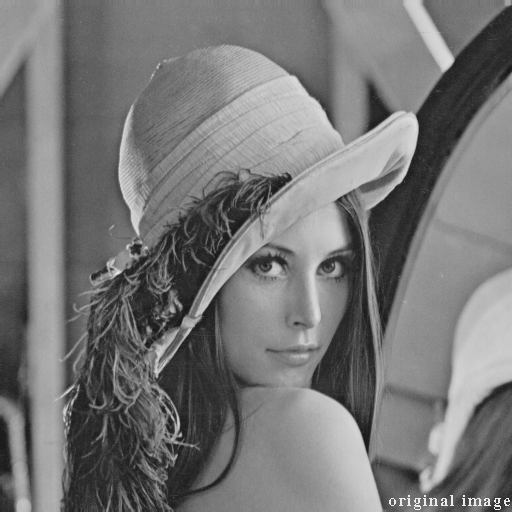
\includegraphics[width=.4\linewidth]{lenaYchannel.png}
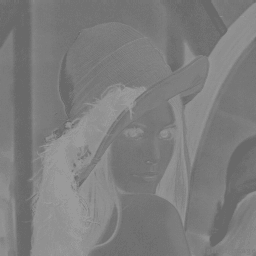
\includegraphics[width=.2\linewidth]{lenaCbchannel.png}
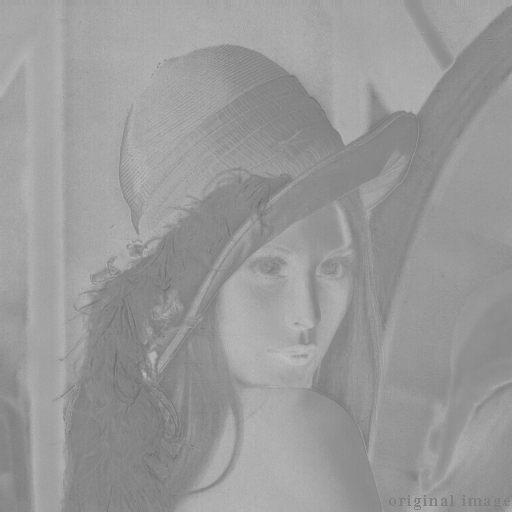
\includegraphics[width=.2\linewidth]{lenaCrchannel.png}
\captionof{figure}{Y, Cb and Cr channels of an image}\label{fig:YCbCrChannels}
\end{centering}

\vspace{4mm}
\subsubsection*{Discrete Cosine Transform}
\vspace{-2.5mm}
After sampling the image, it must be split into blocks called MCUs. The default size of an MCU is 8x8 pixels, but it changes when sampling is used. In the section above, we used a sampling of 4:2:0 where the chroma channels where downscaled by 50\% in both directions. This means that when the sampling of 4:2:0 is used, we have a MCU with a size of 16x16 pixels.

For each 8x8 block of pixels in our MCUs we perform DCT. The two-dimensional DCT is given by:

$$ G_{u,v} = c(u,v)\sum_{x=0}^{7}\sum_{y=0}^{7}g_{x,y}\cos{\left(\frac{(2x+1)u\pi}{16}\right)}\cos{\left(\frac{(2y+1)v\pi}{16}\right)} $$

where:
\begin{itemize}
	\item $u$ is the horizontal spatial frequency 
	\item $v$ is the vertical spatial frequency 
	\item $c(u,v) = \begin{cases}\frac{1}{8} \quad \quad \quad \quad\text{if } u=v=0\\ 
	                             \frac{1}{4 \cdot \sqrt{2}} \,~\quad\quad \text{ if } u = 0 \text{ or } v = 0\\
	                             \frac{1}{4} \quad \quad \quad \quad\text{otherwise}
	                             \end{cases} $
    \item $g_{x,y}$ is the value of pixel at coordinates $(x,y)$ 
\end{itemize}

\vspace{4mm}
\subsubsection*{Quantization}
\vspace{-2.5mm}
Quantization tables are what makes JPEG compression lossy. 
After the DTC process, the quantization progress is performed on the resulting 8x8 block of values.
Quantization is the process of dividing each value in the 8x8 block with a corresponding value in a quantization table. 
The JPEG specification allows 4 quantization tables to be used, while JFIF limits it even further to 2 tables. 
This means that two of our three channels have to share quantization tables. 
As the human eye is much more sensitive to changes in the luminance channel, JFIF specifies that the luminance channel gets its own quantization table, while the chroma components must share a quantization table.

Although the JPEG standard does not force you to use default tables, they do provide some tables which have shown good results with their test images. The proposed quantization table for the image channels are shown below.

\begin{centering}
\hspace{-3mm}\tcbox[left=0mm,right=0mm,top=0mm,bottom=0mm,boxsep=0mm,
toptitle=0.5mm,center title, bottomtitle=0.5mm,nobeforeafter,title=Proposed Quantization Table for Luminance Channel]{
\small
	 	\begin{tabular}{|c|c|c|c|c|c|c|c|}\hline
			16 & 11 & 10 & 16 & 24 & 40 & 51 & 61 \\ \hline
			12 & 12 & 14 & 19 & 26 & 58 & 60 & 55 \\ \hline
			15 & 14 & 16 & 24 & 40 & 57 & 69 & 56 \\ \hline
			14 & 17 & 22 & 29 & 51 & 87 & 80 & 62 \\ \hline
			18 & 24 & 37 & 56 & 68 & 109 & 103 & 77 \\ \hline
			24 & 35 & 55 & 64 & 81 & 104 & 113 & 92 \\ \hline
			49 & 64 & 78 & 87 & 103 & 121 & 120 & 101 \\ \hline
			72 & 92 & 95 & 98 & 112 & 100 & 103 & 99 \\ \hline
		\end{tabular}
}
\tcbox[left=0mm,right=0mm,top=0mm,bottom=0mm,boxsep=0mm,
toptitle=0.5mm,center title, nobeforeafter,bottomtitle=0.5mm,title=Proposed Quantization Table for Chroma Channels]{
\small
	 	\begin{tabular}{|c|c|c|c|c|c|c|c|}\hline
			17 & 18 & 24 & 47 & 99 & 99 & 99 & 99\\ \hline
			18 & 21 & 26 & 66 & 99 & 99 & 99 & 99\\ \hline
			24 & 26 & 56 & 99 & 99 & 99 & 99 & 99\\ \hline
			47 & 66 & 99 & 99 & 99 & 99 & 99 & 99\\ \hline
			99 & 99 & 99 & 99 & 99 & 99 & 99 & 99\\ \hline
			99 & 99 & 99 & 99 & 99 & 99 & 99 & 99\\ \hline
			99 & 99 & 99 & 99 & 99 & 99 & 99 & 99\\ \hline
			99 & 99 & 99 & 99 & 99 & 99 & 99 & 99\\ \hline
		\end{tabular}
}
\end{centering}

\vspace{4mm}
\subsection*{Zigzag-ordering} 
\vspace{-2.5mm}
Because of the quantization process, there are now a lot of zeros in the lower-right corner of the 8x8 block of pixels.
This feature can be utilised to compress the image data, but first the table must be ordered so that the zeros are placed next to each other. 

To do this, the 8x8 block of pixels are now read in a zigzag manner displayed on figure \ref{fig:zigzag}.
By reading the block this way, you have a 64 dimensional vector with a lot of consecutive zeros. 

\begin{centering}
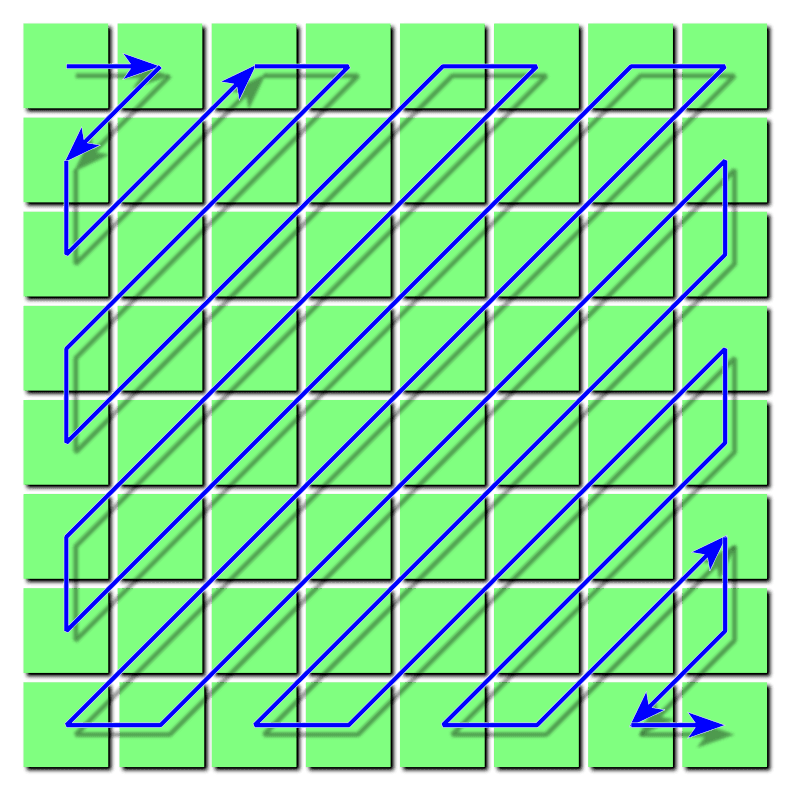
\includegraphics[width=.5\textwidth]{figures/zigzagordering.png}
\captionof{figure}{Zigzag-ordering of the 8x8 block of pixels}
\label{fig:zigzag}
\end{centering} 

\vspace{4mm}
\subsection*{Encoding the vector}
\vspace{-2.5mm}
The first entry in the vector is called the DC coefficient, and will be encoded differently from the other 63. To encode the last 63 entries, run-length encoding (RLE) is used. Each value different from zero in the vector is represented as $(\text{Number of zeros before this entry}, \text{Entry})$. Because of the many consecutive zeros in the data, this allows a very compact encoding of the numbers. If at one point in the vector only zeros remain, we end the block with the EOB value (0,0). 

The DC coefficient is often a large number, so it would be a waste of bits to write it in full to the file each time. Instead only the difference from the previous DC coefficient is stored, so that smaller numbers need to be encoded. So when reading a JPEG file, a decoder must keep track of the previous DC coefficient. The first coefficient encoded, of course, is the whole number.

There are some restrictions to this encoding, as only a nibble is used to represent the number of preceding zeros, the maximum value we can denote is $F_{16}=15_{10}$.
If there are more than 15 consecutive zeros, we can encode 16 zeros as (15,0), and by using multiple of these values, denote any number of consecutive zeros. 

\vspace{4mm}
\subsection*{Huffman Encoding}
\vspace{-2.5mm}
After the run-length encoding, the pairs must be written to the file, but before that can happen, the JPEG standard defines even more compression of the data. Instead of storing the actual values from the vector, a category of the number, along with a bit representation is stored. 

The category of a number is the least amount of bits required to represent the number. The category of numbers in the range $[-32767, 32767]$ are shown in the table below.

\begin{centering}
\resizebox{\textwidth}{!}{%
	\begin{tabular}{|c|c|c|} \hline
		Values & Category & Bit representation \\ \hline
		$0$ & $0$ & - \\
		$-1,1$ & $1$ & $0,1$ \\
		$-3, -2, 2, 3$ & $2$ & $00, 01, 10, 11$ \\
		$-7, -6, -5, -4, 4, 5, 6, 7$ & $3$ & $000, 001, 010, 011, 100, 101, 110, 111$ \\
		$\vdots$ & $\vdots$ & $\vdots$ \\
		$-32767, -32766 \ldots, 32766, 32767$ & $16$ & $0000000000000000 \ldots 1111111111111111$ \\ \hline
	\end{tabular}
	}
\end{centering}

The vector entry of $(0,6)$ would become $(0,(3,110))$ when encoded as shown above. The last step is to Huffman encode these pairs of numbers.
In a 8x8 block of pixels, there may be a lot of $(0,6)$, so instead of having to spend two bytes every time this pair appears, we use Huffman Tables. 

A Huffman Table is a table where you can look up pairs of numbers and get a bit representation which corresponds to the pair of numbers. To complete the example with the entry $(0,6)$ which was encoded to $(0,3,110)$, $(0,3)$ is looked up in the Huffman Table and it can be seen that it has a category of $3$, and a bit representation of $100$. 

So instead of having to write $0000 0000 0000 0110$, which is the byte representation of $(0,6)$, it is enough to write the Huffman encoded $100110$.

There are no universal Huffman tables, and JPEG allows an encoder to define its own. They do, however, provide some Huffman tables which have shown good results with a variety of images \citep[p. 153]{JPEGStandard}. 

\vspace{4mm}
\subsection*{Dissection of a JPEG file}
\vspace{-2.5mm}
In this section a JFIF file which is compatible with the JPEG standard will be explained. The explanation is split into the same segments as the file itself is split into.
\newpage
\subsubsection*{Segments in a JPEG file}
\begin{wraptable}{r}{5.5cm}
\caption{Most commonly used markers in JPEG files}
\label{tab:markers}
\begin{tabular}{|p{2.7cm}|l|}
\hline
Marker & Identifier\\ \hline
0xFFD8 & SOI\\ \hline
0xFFE$n$ \newline$(n = \{0 \ldots F\})$ & APP$n$\\ \hline
0xFFD8 & DQT \\ \hline
0xFFC0 & SOF \\ \hline
0xFFC4 & DHT\\ \hline
0xFFDA & SOS\\ \hline
0xFFD9 & EOI\\ \hline 
\end{tabular}
\end{wraptable}

The JPEG standard defines that a JPEG file must be ordered in segments.
These segments are each indicated by a marker, and the most common segment markers are shown in table \ref{tab:markers}.
Most of the markers are followed by 2 bytes of data describing the length of the following segment.
Knowing the length makes it possible for a decoder to skip segments it does not know how to understand. 

As shown in table \ref{tab:markers}, all markers start with the byte 0xFF.
A special case exists, where 0xFF does not define a marker, and that case is if the following byte is 0x00.
More on this later, when it is examined how image data is written to a file.

\subsubsection*{The SOI and EOI markers}
\begin{centering}
\hspace{1.2cm}\tcbox[left=0mm,right=0mm,top=0mm,bottom=0mm,boxsep=0mm,
toptitle=0.5mm,center title, nobeforeafter, bottomtitle=0.5mm,title=Start of Image Segment]{
	 	\begin{tabular}{|l|l|l|}
			Size in bytes  & Description \\ \hline \hline
			2 bytes  & SOI marker\\ \hline
		\end{tabular}
} \tcbox[left=0mm,right=0mm,top=0mm,bottom=0mm,boxsep=0mm,
toptitle=0.5mm,center title, nobeforeafter,bottomtitle=0.5mm,title=End of Image Segment]{
	 	\begin{tabular}{|l|l|l|}
			Size in bytes  & Description \\ \hline \hline
			2 bytes  & EOI marker\\ \hline
		\end{tabular}
}
\end{centering}\\
The first marker a JPEG decoder meets in a JPEG file is the SOI marker. 
The marker does not specify a length in the following bytes, since the segment only consists of the marker itself.
Likewise, the last marker a decoder will meet is the EOI marker, which specifies that all data has been read from the image.

\subsubsection*{The APP$n$ marker}
\begin{centering}
\tcbox[left=0mm,right=0mm,top=0mm,bottom=0mm,boxsep=0mm,
toptitle=0.5mm,center title, bottomtitle=0.5mm,title=APP$n$ Segment]{
	 	\begin{tabular}{|l|l|l|}
			Size in bytes  & Description \\ \hline \hline
			2 bytes  & APP$n$ marker\\ \hline
			2 bytes & Segment length\\ \hline
			variable & Application specific data
		\end{tabular}
}
\end{centering}
The JPEG standard defines the APP segments to be application specific data, which can be placed anywhere in the image file. Applications can then use these segments to store additional information about the image file. JFIF specifies that the APP$_0$ is used for identifying the file as a valid JFIF file, and that the APP$_0$ segment must be placed immediately after the SOI marker.

By convention the APP$n$ segments use a null terminated string for identifying themselves. The JFIF APP segment as found in almost all JPEG files can be seen in table \ref{JFIFAPP0}.

\begin{centering}
\tcbox[left=0mm,right=0mm,top=0mm,bottom=0mm,boxsep=0mm,
toptitle=0.5mm,center title, bottomtitle=0.5mm,title=JFIF APP$_0$ Segment]{

	 	\begin{tabular}{|l|l|l|}
			Size in bytes  & Value \\ \hline \hline
			2 bytes  & APP$_0$ marker\\ \hline
			2 bytes & Segment length\\ \hline
			5 bytes & Null terminated string ``JFIF''\\ \hline
			2 bytes & Major and minor version number\\ \hline
			1 byte & Units for setting photo density\\ \hline
			4 bytes & X-density and Y-density\\ \hline
			2 bytes & Width and height of thumbnail image\\ \hline
			variable & Thumbnail data saved in RGB colour space.\\ \hline
		\end{tabular}
}

	 	\captionof{table}{JFIF APP$_0$ Segment}\label{JFIFAPP0}
\end{centering}

\subsubsection*{The DQT marker}
\begin{centering}
\tcbox[left=0mm,right=0mm,top=0mm,bottom=0mm,boxsep=0mm,
toptitle=0.5mm,center title, bottomtitle=0.5mm,title=Define Quantization Table Segment]{
	 	\begin{tabular}{|l|l|l|}
			Size in bytes  & Description \\ \hline \hline
			2 bytes  & DQT marker\\ \hline
			2 bytes & Segment length\\ \hline
			4 bits & Quantization value size (0 = 1 byte, 1 = 2 bytes) \\ \hline
			4 bits & Table identifier (0-1) \\ \hline
			64 or 128 bytes & Unsigned quantization values\\ \hline
		\end{tabular}
}
\end{centering}

The Define Quantization Table segment encodes the 8x8 block of integers used in the quantization process. 
The table can use either one or two bytes for storing the integers in the quantization tables. 
Therefore a nibble is used for selecting how many bytes to use.

The JFIF standard allows a JFIF file to use two quantization tables, which means that some channels have to share quantization tables. 
Because of this, each quantization table gets an ID, so that each component can point to a quantization table. 
s
While encoding the actual values of the table, they are encoded top to bottom, left to right.


\subsubsection*{The DHT marker}
\begin{centering}
\tcbox[left=0mm,right=0mm,top=0mm,bottom=0mm,boxsep=0mm,
toptitle=0.5mm,center title, bottomtitle=0.5mm,title=Define Huffman Table Segment]{
	 	\begin{tabular}{|l|l|l|}
			Size in bytes  & Description \\ \hline \hline
			2 bytes  & DHT marker\\ \hline
			2 bytes & Segment length\\ \hline
			4 bits & Table class (0 = DC table, 1 = AC table) \\ \hline
			4 bits & Table identifier (0 or 1) \\ \hline
			16 bytes & A byte for the count of Huffman codes for each length 1-16\\ \hline
			Variable & The one byte codes encoded by the Huffman Table\\ \hline
		\end{tabular}
}
\end{centering}

The Define Huffman Table segment describes how values are encoded in the image data. 
The first part of the segment defines whether the table is used for DC or AC components. Next an ID is defined, so that each channel can be linked to a certain Huffman Table.

The next 16 bytes define how many codes of a certain length are encoded. 
The first byte describes how many codes of length one are encoded, the next how many codes of length two are encoded and so on, until all 16 bytes are used. 

Now, the actual one byte codes which the Huffman Table has to convert, are supplied.
There are as many bytes as the sum of the previous 16 bytes. 
The order in which they are supplied, defines which codes in the Huffman Table they become encoded as.

\subsubsection*{The SOF marker}
\begin{centering}
\tcbox[left=0mm,right=0mm,top=0mm,bottom=0mm,boxsep=0mm,
toptitle=0.5mm,center title, bottomtitle=0.5mm,title=Start of Frame Segment]{
	 	\begin{tabular}{|l|l|l|}
			Size in bytes  & Description \\ \hline \hline
			2 bytes  & SOF marker\\ \hline
			2 bytes & Segment length\\ \hline
			1 byte & Sample precision in bits \\ \hline
			2 bytes & Image height \\ \hline
			2 bytes & Image width \\ \hline
			1 byte & Number of components\\ \hline
		\end{tabular}
}
\end{centering}

The Start of Frame segment defines the components in the frame. 
First, the height and width of the image in pixels are encoded. 
After that, a byte is used for defining the number of following component.
By using a byte for the number of components, the JPEG standard allows a total of $11111111_2=255_{10}$ components, but JFIF limits this to 1 for grey-scale images or 3 for true-colour images.

Next follows a Component Segment for each of the components defined in the SOF segment.
Firstly the segment defines an ID for the component.
Again, JFIF states that we must use the ID 1 for the luminance channel, 2 for the chroma-blue channel and 3 for the chroma-red channel.

Next, each component supplies the scaling of the particular component, both horizontal and vertical.
Lastly, the ID of the quantization table to use for each component is supplied. 

\begin{centering}
\tcbox[left=0mm,right=0mm,top=0mm,bottom=0mm,boxsep=0mm,
toptitle=0.5mm,center title, bottomtitle=0.5mm,title=Component Segment]{
	 	\begin{tabular}{|l|l|l|}
			Size in bytes  & Description \\ \hline \hline
			1 byte & Component identifier (1 = Y, 2 = Cb, 3 = Cr) \\ \hline
			4 bits & Horizontal sampling \\ \hline
			4 bits & Vertical sampling \\ \hline
			1 byte & Quantization table identifier \\ \hline
		\end{tabular}
}
\end{centering}

\subsubsection*{The SOS marker}
\begin{centering}
\tcbox[left=0mm,right=0mm,top=0mm,bottom=0mm,boxsep=0mm,
toptitle=0.5mm,center title, bottomtitle=0.5mm,title=Start of Scan Segment]{
	 	\begin{tabular}{|l|l|l|}
			Size in bytes  & Description \\ \hline \hline
			2 bytes  & SOS marker\\ \hline
			2 bytes & Segment length\\ \hline
			1 byte & Number of components \\ \hline
			2 $\cdot$ ``Number of components'' bytes & Scan component descriptor \\ \hline
			1 byte & Spectral selection start\\ \hline
			1 byte & Spectral selection end \\ \hline
			1 byte & Successive approximation\\ \hline
		\end{tabular}
}
\end{centering}
The Scan Segment is where the actual image information is stored. First we have the Start of Scan segment which is a fixed length segment describing what image data will follow. Again the segment describes how many components to encode, then for each component supplies their Scan Component Descriptor which contains an ID for the component, together with the linked Huffman Tables for the DC and AC components.

\begin{centering}
\tcbox[left=0mm,right=0mm,top=0mm,bottom=0mm,boxsep=0mm,
toptitle=0.5mm,center title, bottomtitle=0.5mm,title=Scan Component Descriptor Segment]{
	 	\begin{tabular}{|l|l|l|}
			Size in bytes  & Description \\ \hline \hline
			1 byte & Component identifier \\ \hline
			4 bits & DC Huffman Table identifier\\ \hline
			4 bits & AC Huffman Table identifier\\ \hline
		\end{tabular}
}
\end{centering}

\vspace{4mm}
\subsubsection*{The scan data}
\vspace{-2.5mm}
After the SOS segment, the scan data follows, which is the actual image information.
The data is not preceded by any marker.
This is where the Huffman encoded data is written, and is the data that the image processors use for calculating the actual pixel's colours.

In the beginning of this section it was explained that a marker with the name FF00 does not exist.
The reason for this is that if the scan data must encode the byte $1111 1111_2=\text{FF}_{16}$. 
It cannot do so without it being read as a marker.
Therefore the JPEG specification reads that two consecutive bytes $\text{FF}00$ must be read as $\text{FF}$ and not as a marker. 

\end{infobox}